\documentclass{article}
\usepackage{fullpage}
\usepackage{amsmath, amssymb}
\usepackage[hidelinks]{hyperref}
\usepackage[utf8]{inputenc}
\usepackage{natbib}
\usepackage{graphicx}
\usepackage{enumitem}
\usepackage{listings}
\bibliographystyle{plainnat}
% \usepackage[T1]{fontenc}


\newcommand{\R}{\mathbb{R}}
\newcommand{\Q}{\mathbb{Q}}
\newcommand{\Z}{\mathbb{Z}}
\newcommand{\N}{\mathbb{N}}
\newcommand{\C}{\mathbb{C}}

\renewcommand{\P}{\mathbb{P}}
\newcommand{\E}{\mathbb{E}}
\newcommand{\var}{\mathop{\mbox{Var}}}
\newcommand{\cov}{\mathop{\mbox{cov}}}
%\newcommand{\det}{\mathop{\mbox{det}}}
\newcommand{\supp}{\mathop{\mbox{supp}}}
\newcommand{\sgn}{\mathop{\mbox{sgn}}}
\newcommand{\EE}[1]{\E\!\left[#1\right]}
\newcommand{\PP}[1]{\P\!\left\{#1\right\}}
\newcommand{\PPP}[2]{\P_{#1}\!\left\{#2\right\}}
\newcommand{\EEE}[2]{\E_{#1}\!\left[#2\right]}
\newcommand{\EEsup}[2]{\E^{#1}\!\left[#2\right]}

\newcommand{\bone}{\mathbf{1}}

% These macros are borrowed from TAOCPMAC.tex
\newcommand{\slug}{\hbox{\kern1.5pt\vrule width2.5pt height6pt depth1.5pt\kern1.5pt}}
\def\xskip{\hskip 7pt plus 3pt minus 4pt}
\newdimen\algindent
\newif\ifitempar \itempartrue % normally true unless briefly set false
\def\algindentset#1{\setbox0\hbox{{\bf #1.\kern.25em}}\algindent=\wd0\relax}
\def\algbegin #1 #2{\algindentset{#21}\alg #1 #2} % when steps all have 1 digit
\def\aalgbegin #1 #2{\algindentset{#211}\alg #1 #2} % when 10 or more steps
\def\alg#1(#2). {\medbreak % Usage: \algbegin Algorithm A (algname). This...
  \noindent{\bf#1}({\it#2\/}).\xskip\ignorespaces}
\def\kalgstep#1.{\ifitempar\smallskip\noindent\else\itempartrue
   \hskip-\parindent\fi
   \hbox to\algindent{\bf\hfil #1.\kern.25em}%
   \hangindent=\algindent\hangafter=1\ignorespaces}

\newcommand{\algstep}[3]{\kalgstep #1 [#2] #3 }
\newenvironment{taocpalg}[3]{%
\vspace{1em}%
\algbegin Algorithm #1. ({#2}). #3 }
{\vspace{1em}}

\newcommand{\randomuniform}[0]{\mathcal{R}_U}
\newcommand{\randomdiscrete}[0]{\mathcal{R}_D}
\newcommand{\algref}[1]{#1}

% \newcommand{\tablenotation}[1]{\mathcal{#1}}
% \newcommand{\tableaddrow}[0]{\mbox{add}}


\newcommand{\msprime}{\texttt{msprime}}
\newcommand{\nodes}{\texttt{nodes}}
\newcommand{\edgesets}{\texttt{edgesets}}
\newcommand{\sites}{\texttt{sites}}
\newcommand{\mutations}{\texttt{mutations}}

\usepackage{color}
\newcommand{\plr}[1]{{\em \color{blue} #1}}
\newcommand{\jk}[1]{{\em \color{red} #1}}

\begin{document}

\title{Efficient forwards-time simulation with ancestral recombination graphs}
\author{Jerome Kelleher,
        Kevin R. Thornton,
        Jaime Ashander, and
        Peter L. Ralph}
\maketitle

\emph{Note:} author order not determined

\begin{abstract}
    To use genomic data for inference and prediction
    it is often necessary to obtain whole-genome information
    from individual-based simulations,
    but the computational burden of tracking the genome of each simulated individual can be substantial.
    In this note we describe how to both (a) dramatically reduce this burden and
    (b) efficiently record the entire history of the population.
    We do this by simulating only those loci that may affect reproduction (those having non-neutral variants),
    and recording the entire history of genetic inheritance in an efficient representation of the ancestral recombination graph,
    on which neutral mutations can be quickly placed afterwards.
    \plr{make more clear data structure was already developed? refer to 'tree sequence' by name?}
    The algorithm is implemented in python,
    and is designed to be easily used by any forwards-time simulation software.

    Coalescent simulations are very helpful but require random mating and neutrality.
    For continuous space, polygenic selection, or detailed dissection of life history,
    we must use forwards-time, individual-based simulation.
    These are much slower due in part to carrying around neutral genotypes irrelevant to the process.
    Here we show how to efficiently produce and store the entire history of ancestry and recombination
    from an individual-based simulation,
    on which neutral mutations can be placed afterwards.
    This has the promise of making large-scale, whole-genome simulations with realistic geography and selection finally possible.
\end{abstract}


\textbf{OUTLINE}
\begin{enumerate}
    \item motivate need for whole-genome fwd-time simulations; point out that we only recently have the computing power to do this
    \item explain ARG: explain that for forwards-time only need selected loci as by defn all others can be put on afterwards
    \item review something about msprime methods for storing/traversing tree sequence
    \item describe tables and write out conditions to have valid tables
    \item write down algorithm used to do simple WF simulation
    \item describe simplify algorithm
    \item back-of-the-envelope calculation to compare cost of tracking whole genomes versus putting mutations on ARG
    \item comparison of speed with simupop, fwdpp
\end{enumerate}


%%%%%%%%%%%%%%%%%%%%%%
\section*{Introduction}

\plr{perhaps some of this veers into methods rather than introduction}

Since the 1980's, coalescent theory has enabled computer simulation of the results of population genetics models
identical to that which would be produced by large, randomly mating populations over long periods of time
without actually requiring simulation of so many generations or meioses.
Coalescent theory thus had three transformative effects on population genetics:
first, giving researchers better conceptual tools to describe \emph{gene trees} and thus bringing within-population trees into better focus;
second, producing analytical methods to estimate parameters of interest from genetic data (e.g.\ $\theta = 4N_e \mu$);
and finally, providing a computationally feasible method to produce computer simulations of population genetics processes.
However, these powerful advances came with substantial caveats:
the backwards-in-time processes that are described by coalescent theory
are only \emph{Markovian}, and thus feasible to work with,
thanks to the important assumptions of (a) random mating, and (b) neutrality.
\plr{Brief statement why this is.  Also include stationarity?}
Both assumptions can be side-stepped to a limited extent, and so coalescent methods are now commonly used to
simulate the results of population dynamics of a collection of randomly mating populations exchanging migrants,
having a small number of loci under selection.
Mapping results of such models onto real species can be challenging,
as these are often distributed across geographical space and may have large numbers of loci under various sorts of selection.
Furthermore, the relationship between the life history of a species --
fecundity and mortality schedules, allee effects, and demographic fluctuations --
are all absorbed into a single compound parameter, the coalescence rate.
These considerations, and increasing computational power, have led to a resurgence of interest in forwards-time, individual-based simulations.

Another critical assumption of the coalescent is that the sample size $n$ is much smaller
than the effective population size $N_e$. With the very large sample sizes becoming common
in human genetics, this is no longer a safe assumption. For example, a recent study~\citep{martin2017human}
simulated 600,000 samples of human chromosome 20 to assess the impact of European biased
reference panels in genome wide association studies. While many results of the
coalescent are surprisingly
robust to violations of the assumption that $n \ll N$, there are instances where genealogical properties
are distorted and coalescent simulations may be
misleading~\citep{wakeley2003gene,maruvka2011recovering,bhaskar2014distortion}.
A hybrid approach, in which the recent history of a large sample of
individuals is simulated under a detailed forwards-in-time model and the deep history
under the coalescent, is an attractive prospect.
\jk{Not sure where this should go; perhaps in the discussion? We can make the point that
by keeping track of the genealogies forwards in time we can easily combine these with the
deep history simulated by msprime}

With modern computing power, pure demographic calculations are not a barrier,
even though biological population sizes are often above $10^6$,
and coalescent theory tells us that a population of size $N$
must be run for a multiple of $N$ generations to produce stable genetic patterns.
However, if our interest lies in the resulting genetic patterns of variation
-- and often, the point of such simulations is to compare to real data --
then such simulations must somehow produce at the end data for each individual on a genomic scale.
As samples of most species genomes harbor tens or hundreds of millions of variant sites,
naively carrying full genotypes for even modest numbers of individuals through a simulation becomes quickly prohibitive.

However, it is thought that much of that variation is selectively neutral (or nearly so).
By definition, the alleles carried by individuals in a population at neutral sites
do not affect the population process.
For this reason, if one records the entire genealogical history of a population over the course of a simulation,
one can lay down neutral mutations on top of that history afterwards,
without loss of generality.
Precisely, we would need to know the genealogical tree relating all sampled individuals
at each position along the genome.
In this paper, we show how to use algorithmic tools and data structures developed for the coalescent simulator \msprime\
to efficiently record, and later process, this history.

In so doing we record the \emph{population pedigree} --
the entire history of parent-offspring relationships of an entire population going back to a remote time --
as well as information encoding the genetic outcomes of each ancestral meiosis --
who inherited which parts of which parental chromosomes.
This embellished pedigree contains all the information necessary
to construct the genealogical tree that relates each individual to each other
at each position on the genome, i.e., the \emph{tree sequence}.
Combined with ancestral genotypes and the origins of new mutations,
it also completely specifies the genomic sequence of any individual in the population at any time.
This is much more than we need to know, however,
so we discard all information irrelevant to the genetic history
of the \emph{sampled} individuals,
which results in considerable savings.

Another way of representing this same information
is known as the \emph{ancestral recombination graph}, or {ARG} \citep{griffiths1997ancestral},
which has been the subject of substantial study
under the assumptions of coalescent theory \citep{wiuf1997number,wiuf1999ancestry,marjoram2006coalescent,wilton2015smc}.


%%%%%%%%%%%%%%%%%%%%%%
\section*{Methods}

\plr{Reminder of what we need to know in the end (the trees), and
    quick review of \msprime{} methods: sparse trees, tree differences.}

%%%%%%
\subsection*{Tree sequences}

A tree sequence is an efficient encoding for a sequence of correlated trees such as
is produced by recombination. The encoding is efficient because branches that are
shared by adjacent trees are stored once, rather than repeatedly for each tree.
The topology of a tree sequence is defined via a set of \emph{nodes} and
\emph{edges}. A node in a tree sequence refers to a distinct ancestor and
corresponds to the vertices in the individual genealogies along the sequence.
Since each node represents a specific ancestor, it has a unique ``time'',
thought of as her birth time, which determines the height of any vertices
she is associated with. In the example of Figure~\ref{fig:example_tree_sequence}
we have a total of five nodes. Nodes 0, 1 and 2 occur at time 0 and are our
samples. Nodes 3 and 4 represent the ancestors of these samples, and were born at
time 1.5 and 2.5 respectively.

\begin{figure}
    \begin{center}
        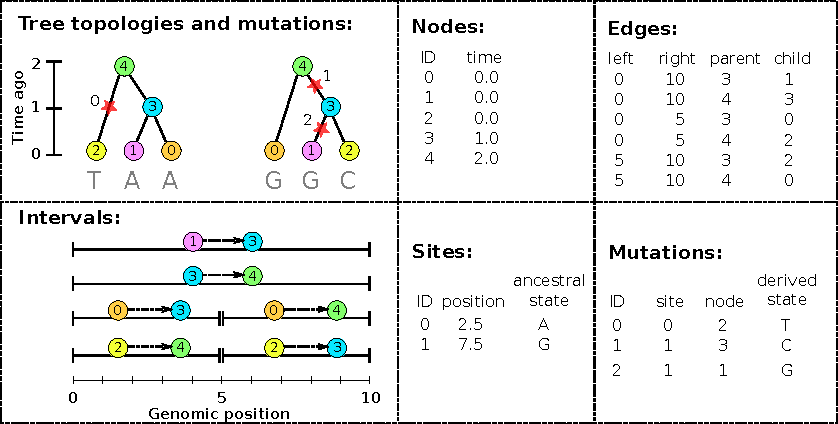
\includegraphics[width=\textwidth]{example_tree_sequence}
    \end{center}
    \caption{
        An example tree sequence with three samples over a chromosome of length 10. In the
        left-most panel we show the tree sequence pictorially in two different ways:
        in the top are the tree topologies and the bottom shows the spatial extent of the
        edges that define these topologies. The right-hand panels show the specific encoding
        of this tree sequence in the four tables (nodes, edges, sites and mutations) defined
        by \msprime.
        \jk{Some minor alignment issues present here.}
        \label{fig:example_tree_sequence}
    }
\end{figure}

The topology of a tree sequence is defined by the \emph{edges} which define how
nodes relate to each other over specific genomic intervals. Each edge is a tuple
$(\ell, r, p, c)$, where $[\ell, r)$ is a half-open genomic interval defining the
spatial extend of the edge; $p$ and $c$ are the parent and child nodes specifying
a single branch in the tree over this interval. The spatial extent of the
edges defining the topology of Figure~\ref{fig:example_tree_sequence} in the
bottom left panel. For example, the branch joining nodes 1 to 3 is shared in both trees,
and is recorded in a single edge extending over the whole chromosome. It is this
method of capturing the shared structure between adjacent trees that makes the
tree sequence encoding very compact and algorithmically efficient.

Recovering the sequence of trees from a collection of edges is straightforward:
each point along the genome that the tree topology changes
is accompanied by the end of some \emph{edges} and the beginning of others.
Since each \emph{edge} records the genomic interval 
over which a given node inherits from a particular ancestor,
to construct the tree at a certain point in the genome
we need only retrieve all edges overlapping that point
and construct the corresponding edges.
To construct the tree at a nearby location,
we need only remove those edges whose intervals do not overlap that location,
and add those new edges whose intervals do.
Incidentally, this property that edges naturally encode \emph{differences}
between nearby trees (e.g., as ``subtree prune and regraft'' moves)
allows for efficient algorithms that take advantage
of the highly correlated nature of nearby trees.

Given the topology defined by the nodes and edges, \emph{sites} and \emph{mutations}
encode the sequence information for each sample in an efficient way. Each site
is associated with a position on the genome and an ancestral state. For example,
in Figure~\ref{fig:example_tree_sequence} we have two sites, one at position
2 and ancestral state `A' and the other at position 7 with ancestral state `G'. If
no mutations occur, all samples inherit the ancestral state at a given site.
A mutation occurs over a specific node at a given site, and results in a specific
derived state. Thus, all samples below the mutation node in the tree will inherit
this state (unless further mutations are encountered). Three mutations are shown
in Figure~\ref{fig:example_tree_sequence}, illustrated by red hexagons. The first
mutation occurs at site zero (which is in the left-hand tree), which is a simple
mutation resulting in node $2$ inheriting the state 'T'. The second side (in the
right hand tree) has two mutations: one occurring over node $3$ changing the state to
`C' and a back mutation over node $1$ changing the state to `G'.

This encoding of a sequence of trees and accompanying mutational information is
very concise. To illustrate this, we ran a simulation of $500,000$ samples of a
$200$ megabase human-like chromosome ($N_e=10^4$ and per-base mutation and
recombination rates of $10^{-8}$ per generation) using \msprime. This resulted
in about 1 million distinct marginal trees and $1.1$ million infinite-sites
mutations. The HDF5 file encoding the nodes, edges, sites and mutations (as
described above) for this simulation consumed 157MiB of storage space. Using
the \msprime\ Python API, the time required to load this file into memory was
around 1.5 seconds, and the time required to iterate over all 1 million tree
was 2.7 seconds. In contrast, recording the topological information in Newick
format would require around 20 TiB and storing the genotype information
in VCF would require about 1 TiB. Working with either the Newick or VCF encoding
of this dataset would be exceedingly cumbersome, likely requiring several
days of CPU time simply to read the information info memory.


%%%%%%
\subsection*{Recording the pedigree in forwards time}

To record the genealogical history of a forwards in time simulation
we need to record two things for each new chromosome:
the birth time, and the endpoints and parental IDs of each distinctly inherited segment.
For concreteness, here we write out in pseudocode how to run a neutral Wright--Fisher simulation
with overlapping generations that records genealogical history in this way.
The simulation will run for $T$ generations,
and has $N$ haploid individuals, each carrying a single chromosome of length L.
For simplicity we assume there is exactly one crossover per generation.
The probability of death per individual each generation is $\delta$.

Let $\randomuniform(A)$ to be an element of the set $A$ chosen
uniformly at random (note that each instance of $\randomuniform(A)$ within
an algorithm listing represents an independent draw from the set $A$).

\begin{taocpalg}{W}{Forwards-time tree sequence}
{Runs a forwards time Wright--Fisher simulation of a populations with $N$
individuals with a probability of death per generation $\delta$ and a chromosome of length
$L$ for $T$ generations. On termination, there will be $n$ nodes with times recorded
in the vector $\tau$, and $E$ will contain a set of $(\ell, r, p, c)$ tuples
describing the recorded edges.
}

\algstep{W1.}{Initialisation.}{
 For $0 \leq j < N$, set $P_j \leftarrow j$ and $\tau_j \leftarrow T$.
Set $E\leftarrow \emptyset$, $t \leftarrow T$ and $n \leftarrow N$.
}

\algstep{W2.}{Generation loop.}{ If $t = 0$ terminate.
Set $P'_j \leftarrow P_j$ for $0\leq j < N$ and then set $t \leftarrow t - 1$ and $j \leftarrow 0$.
}

\algstep{W3.}{Individual loop.}{ If $j = N$ set $P \leftarrow P'$ and go to \algref{W2}.
}

\algstep{W4.}{Mortality.}{ If $\randomuniform([0, 1)) \geq \delta$ go to \algref{W8}.
}

\algstep{W5.}{New node.}{Set $P'_j \leftarrow n$ and $\tau_n \leftarrow t$.
}

\algstep{W6.}{Choose parents.}{Set $a \leftarrow \randomuniform(\{0, \dots, N - 1\})$,
    $b \leftarrow \randomuniform(\{0, \dots, N - 1\})$ and $x \leftarrow \randomuniform([0, L))$.
}

\algstep{W7.}{Record edges}{Set $E \leftarrow E \cup \left\{ (0, x, P_a, n), (x, L, P_b, n) \right\}$
    and $n \leftarrow n + 1$.
}

\algstep{W8.}{Loop tail}{Set $j \leftarrow j + 1$ and go to \algref{W3}.
}

\jk{I haven't checked this carefully. If we used 1-based indexes it might make things a bit
simpler}.
\end{taocpalg}

Algorithm~\algref{W} is a very simple implementation of a Wright--Fisher model
intended to illustrate how we can record the nodes and edges of a tree sequence
forwards in time. We begin in~\algref{W1} by allocating our initial population $P$
and creating $N$ nodes with birth time $T$ generations ago, recorded in the
vector $\tau$. The set $E$ is used to store the edges that we output during the
simulation, and $n$ is the number of nodes created so far (and so, the ID of
the next node we create). Steps~\algref{W2} and~\algref{W3} simply loop over
the generation clock $t$ and individual index $j$. In~\algref{W4} we check if
an individual $P_j$ has died in this generation. If it has, we replace it in
steps \algref{W5}--\algref{W7}; if not, we proceed immediately to the next
individual. When an individual in the population dies, we first allocate
a new node with ID $n$ in~\algref{W5} and record its birth time. Then,
in step~\algref{W6} we choose two indexes $a$ and $b$ uniformly (giving us
parents $P_a$ and $P_b$) and choose a breakpoint $x$. We record the effects of this
event by storing two new edges: one recording that the parent of node $n$
from $0$ to $x$ is $P_a$, and another recording that the parent of $n$
from $x$ to $L$ is $P_b$. We then complete the replacement event by incrementing
$n$, ready to represent the next new node.

This algorithm records only the topological information resulting from the
forwards in time Wright-Fisher process, but it is straightforward to add
mutational information. This can be done in two different ways.
We can record mutations that occur during the simulation quite simply.
For example, in Algorithm~\algref{W} we would generate mutations after
we have recorded the edges joining the new node $n$ to its parents
$P_a$ and $P_b$ in step \algref{W7}.
For example, if we assume that infinite sites mutations
occur at rate $\mu$ per generation then there are $\mbox{Poisson}\left((r - \ell)(\tau_p
- \tau_c)\right)$ mutations on each edge $(\ell, r, p, c)$. Each of these mutations
will occur on a distinct site $x$ drawn uniformly from $(\ell, r]$ and be over node $c$.
It is straightforward to record this information during the simulation, but it
is significantly simpler and more efficient to generate these mutations
after the simulation has completed. In the case of infinite sites mutations
there is no difference between generating these mutations during the forwards
in time simulation and after it has completed. We are using precisely the same
information.

\begin{figure}
    \begin{center}
        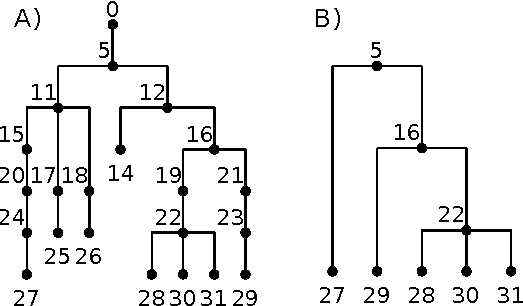
\includegraphics{wf-before-after}
    \end{center}
    \caption{An example of a marginal genealogy from a Wright-Fisher simulation
    with $N=5$. \textbf{(A)} the original tree including all
    intermediate nodes and dead-ends, and \textbf{(B)} the minimal tree
    relating all of the currently-alive individuals (27--31).
    \label{fig:wf-trees}
    }
\end{figure}

It is significantly more efficient to generate mutations as a separate process
after the topological simulation has completed because we will generate many
mutations that will be lost in the population. Figure~\ref{fig:wf-trees} shows
an example of a marginal genealogy produced by a forwards-time Wright-Fisher
process like Algorithm~\algref{W}. There are two different trees in this
figure: one shows all the edges output by the simulation and the other
is the minimal tree representing the ancestry of the currently alive
population. Clearly there is a great deal of redundancy in the topological
information output by the simulation.

There are two sources of redundancy here. The first type of redundancy arises
from nodes in tree that have only one child. In Algorithm~\algref{W} we do
not attempt to track coalescence events but simply record all parent-child
relationships in the history of the population. As such, my of these edges
will record the simple passing of genealogical information from parent to child
and only some small subset will correspond to coalesences within the marginal
trees. The second source of redundancy in the output of Algorithm~\algref{W}
is due to the fact that lineages die out: there will be a large number of
individuals in the simulation that leave no ancestors in the present day
population. Node 26 in Figure~\ref{fig:wf-trees}a, for example, leaves no
ancestors in the current population and so the entire path tracing back to
the root is redundant.

One of the reasons that it is more efficient to generate mutations on the
genealogies after we have completed the forwards in time simulation is
because we avoid the cost of generating mutations on these dead-end branches.
It is only with the benefit of hindsight that we can know which lineages end
up being ancestral to the sample, and we can avoid a substantial cost of
generating and maintaining mutational information on these evolutionary
dead-ends. Assuming mutations are rare, another  reason that it is more efficient
to place mutations on the trees afterwards is that we have far fewer edges
in the trees: because we have removed all the intermediate `unary' nodes, we
have fewer edges to generate mutations on.

There are many advantages to having minimal genealogies such as show in
Figure~\ref{fig:wf-trees}. Computing this minimal representation of the
edges output by a forward-time simulation is an instance of a more
general problem that we refer to as `tree sequence simplification'. We discuss
this problem and an efficient solution in the next subsection.

%%%%%%
\subsection*{Tree sequence simplification}

Suppose we have a tree sequence consisting of a set of nodes and edges as
described earlier, and we have some subset of the nodes in this tree sequence
that we are interested in (our `samples').  We wish to reduce the input tree sequence
into the minimum representation of the topologies that include the specified
samples. The output tree sequence must have the following properties:
\begin{enumerate}
\item we must have the same marginal trees with respect to the samples as
the input;
\item within the marginal trees, all non-sample vertices must has at least
two children (i.e., unary tree vertices are removed);
\item any nodes and edges not reachable from the sampled nodes are removed;
\item there are no adjacent redundant edges, i.e, pairs of edges $(\ell, x, p,
c)$ and $(x, r, p, c)$ which can be represented with a single edge
$(\ell, r, p, c)$.
\end{enumerate}

\begin{figure}
    \begin{center}
        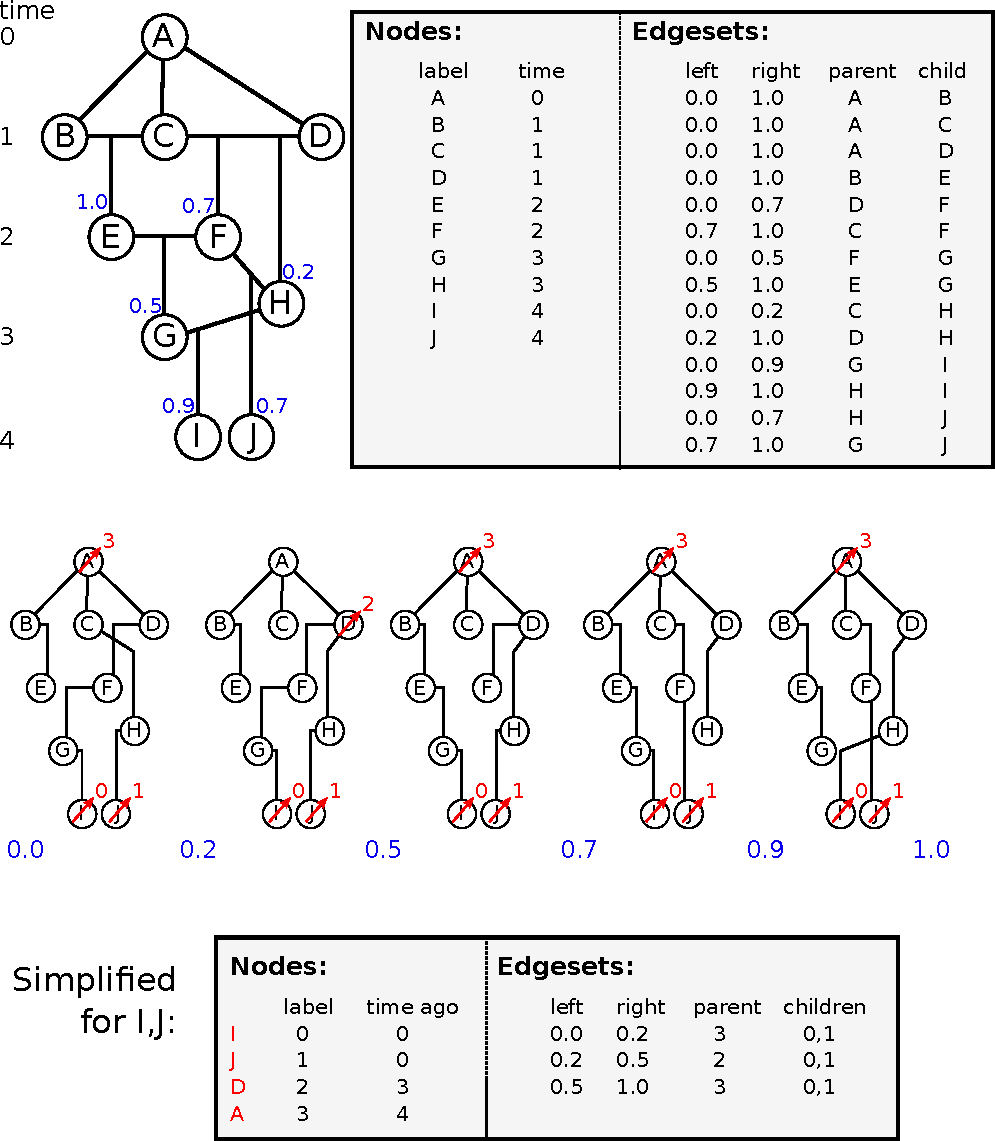
\includegraphics{method_diagram}
    \end{center}
    \caption{
        A simple example of the method.
        \textbf{Top:} the diagram on the left relates ten haploid individuals to each other.
        It is recorded, in forwards time,
        in 10 node records (one for each individual)
        and 14 edge records (one for each distinctly inherited segment).
        Blue numbers denote crossing over locations in each meiosis.
        The individuals $B$, $C$, and $D$ inherit clonally from $A$.
        \textbf{Center:} the five distinct trees relating all individuals to each other
        found across the chromosome (blue numbers denote locations on the chromosome).
        Labels after simplification are shown in red.
        \textbf{Bottom:} tables recording the tree sequence after simplification
        with nodes $I$ and $J$ as samples.
        The mapping from labels in the forwards time simulation to nodes in the tree sequence
        is shown in red,
        which allows additional records to be added as the simulation progresses.
        \label{fig:method_diagram}
    }
\end{figure}

In the current context of running forwards in time simulations, the tables of
nodes and edges that we record all of history for everyone alive at any time through the simulation.
This is much more than we need to reconstruct the genealogies and sequences
of the current day population. We can use the process of simplification here to
reduce this down to the minimal set of nodes and edges required to represent
the information that we are interested in. We can also use simplification if  we have some very
large tree sequence representing a large dataset and we wish to extract the
information relevant to a subset of the samples.

Roughly, simplification works by tracing ancestry from the samples backwards
through the recorded history, adding node and edge records to the output
only when coalescent events are reached. This works exactly as in \msprime,
allowing substantial re-use of algorithms; the main difference being that
parental choice, mutations, and recombination locations are determined by the
input tree sequence rather than randomly generated. An example is shown in
Figure \ref{fig:method_diagram}.

\begin{figure}
    \begin{center}
        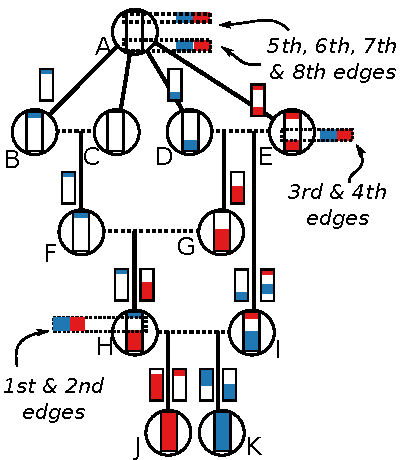
\includegraphics{simplify-state-diagram}
    \end{center}
    \caption{
        A depiction of the state of the simplification algorithm.
        \label{fig:simplify_state}
    }
\end{figure}

The approach that we take is based on Hudson's algorithm for simulating
the coalescent with
recombination~\citep{hudson1983properties,kelleher2016efficient}. The main
state of the algorithm is a set of ancestral segments; each segment $(\ell, r,
u)$ represents a tract of ancestral material in which the node $u$ is
associated with the genomic interval $[\ell, r)$. In the same manner
as Hudson's algorithm, we represent the set of extant lineages as a
set of individuals, where each ancestral individual is composed of a
linked list of these segments. The node $u$ in each ancestral sequence
is the node ID associated with this segment in the output tree sequence.
We maintain a map $A$ such that $A_j$ is segment chain for node $j$ in
the input tree sequence.

\jk{I'm not sure this is the right level of detail to tackle this description
at. What's the goal of this algorithm description? Are we trying to
establish some properties of the algorithm or just give the reader a high-level
flavour of how it works??}

In this scheme, at any point in the simulation genealogical history is recorded
in a tree sequence. This has two additional advantages. First, simplification
can be run periodically through the simulation, taking the set of samples to be
the entire currently alive population. This is important as it keeps memory
usage from growing linearly (and quickly) with time. Second, the simulation can
be \emph{begun} with a tree sequence produced by some other method -- for
instance, by a coalescent simulation with \msprime. This allows for
incorporation of deep-time history beyond the reach of individual-based
simulations. Since geographic structure from times longer ago than the mixing
time of migration across the range has limited effect on modern genealogies
\citep{wilkins_separation} (other than possibly changing effective population
size \citet{durretspatial}), this may not negatively affect realism.


%%%%%%
\subsection*{Overview of the API}

The \msprime\ Python API provides a powerful platform for working with
tree topology and mutation data. We refer to the part of \msprime\
that is dedicated to tree sequence input and output as the `Tables API',
as the API is organised around simple tables of data. There are four key
tables: nodes, edges, sites and mutations. Briefly, nodes and edges define
the topology of a tree sequence (as defined above) and the sites and mutations
define mutational processes on this topology.
Figure~\ref{fig:example_tree_sequence} gives an informal depiction of this
encoding in terms of these tables.

The tables API is primarily designed to facilitate efficient interchange of
data between programs or between different modules of the same program.
Following the current best-practises [citations: apache arrow, etc] data is stored
in a columnar format. There are many advantages to this approach, but the
principle advantage for our purposes is that it allows for very efficient
interchange of large amounts of numerical data. In principle, this enables
zero-copy semantics, where a data consumer can read the information directly
from the memory of a producer without incurring the overhead of a copy
[citation?] Our implementation uses the numpy C API [citation] to efficiently copy
data from Python into the low-level C library used to manipulate
tree sequences.

The tables API provides basic input and output operations via the numpy
array interface, which provides a great deal of flexibility as well
as efficiently. This makes transferring data from various sources
such as HDF5 [citation], Dask, Zarr etc, straightforward. (For small
scale data and debugging purposes, a simple text format is also supported.)
Along with
these operations we also provide a function to sort a set of tables
to ensure that the records are in the form required to input
into an \msprime\ tree sequence object. The \texttt{simplify\_tables}
function implements tree sequence simplification, as described in the
previous subsection.

This interchange API is very efficient. [Describe a quick example where we generate
a many-gigabyte tree sequence using fwdpp, and the time required
to copy the node and edge data into the tables]. By using a simple numerical
encoding of tree topologies and contiguous arrays of data to store this
encoding, we can achieve data transfer rates that would be impossible under
any text-based approach while retaining excellent portability.

%%%%%%%%%%%%%%%%%%%%%%
\section*{Results}

\plr{Estimates of run-time complexity}
Suppose that we wish to run a forwards-time simulation of $N$ individuals for $T$ generations,
in which there are $S$ selected loci and $L$ neutral loci using a similar
method to Algorithm~\algref{W}.
We will estimate run-time complexity and memory usage for both a ``naive'' strategy that carries along neutral loci
and an ``ancestry-tracking'' strategy like that we consider here.
To do this, we assume that each individual must carry along its entire genotype.
More advanced schemes are used in some simulators,
but these increase efficiency by utilizing redundancy introduced by shared ancestry,
which is effectively an intermediate scheme.
We omit the cost of computing a fitness function.

Both schemes must choose mates and recombination breakpoints,
and pass on selected genotypes.
The difference between the two comes from the tradeoff between
(a) passing on neutral genotypes, and
(b) recording and simplifying the tree sequence, and adding neutral genotypes afterwards.
(We assume here that selected genotypes are stored in the same way for both.)
Passing on neutral genotypes naively records $L$ items per individual each
generation, discarding the previous generation, giving an overall complexity of
$O((L + S) NT)$. Tracking the $S$ selected loci and recording a tree sequence
using Algorithm~\algref{W} requires $O(SNT)$ time and space, since we
record at most two edges for each individual in each generation.
However, after simplification the tree sequence contains
$O(??)$ edges since []. The cost of generating $L$ neutral mutations
is then $O(L + ??)$. Assuming that $N$, $T$ and $L$ are large, this is
very much smaller than the straightforward $O((L + S) NT)$ time required
to simulate all mutations directly.

\jk{Not sure where $\rho$ comes in here now. Thinking about this, shouldn't we
be able to come up with some expression for the number of edges? Assuming
the very simple single breakpoint per generation of Alg W, what is the
expected number of breakpoints? This is a function of $N$ and $T$, right?
It's not clear to me how many breakpoints this ends up giving you in
the output tree sequence and how many edges this corresponds to.
It's probably worthwhile thinking about this a bit.}

% However, after simplification a tree sequence for all $N$ individuals
% only takes of order $N + \rho \log N$ records.
% Simplification requires processing each of the initial records -- so, order of $N \times T \times \rho$ operations;


% \begin{table}
% \begin{center}
%     \begin{tabular}{l||r|r||r|r|}
%                     & \multicolumn{2}{|c|}{naive} & \multicolumn{2}{|c|}{ancestry-tracking} \\
%                     & operations  & memory & operations  & memory \\
%         mate choice & $N$       &   --  &   $N$     & -- \\
%         recombination & $N\rho$ &   --  &   $N\rho$ & -- \\
%     \end{tabular}
% \end{center}
% \end{table}

Comparison of simulation with/without msprime, using simuPOP
or maybe just a simple haploid simulation with 1000 QTL and stabilizing selection on a trait (say).

Maybe an estimate of how long \emph{just} the ARG recording and simplification takes,
so that then we can say how fast the simulator would have to be to do $10^6$ whole chromosomes for $10^7$ generations
in a day.

%%%%%%%%%%%%%%%%%%%%%%
\section*{Conclusion}

This works great and very fast.

Having results in a tree sequence is really good downstream too:
The tree sequence encoding is compact but it is also efficient to process.
Many algorithms to compute statistics of interest for population genetics
are naturally expressed in terms of tree topologies. For example, the
pairwise nucleotide diversity $\pi$, is defined as the average number of
differences between sequences in the sample. Computing $\pi$ directly
from observed sequence data requires $O(n^2 m)$ time, since we must
compare all pairs of samples at every site. However, given the topology of
the trees at every site and the locations of mutations much better algorithms
are possible. Using the fact that we can count the number of samples below
a given node efficiently using previously described tree sequence
algorithms~\citep{kelleher2016efficient}, the time required to compute $\pi$
becomes roughly $O(n \log n + m)$.
The \msprime\ API provides a method to compute $\pi$ among arbitrary subsets of the
samples in a tree sequence, and calculating $\pi$ over all 500K samples
in the example above required about 1.2 seconds.
\jk{I haven't checked the analysis of computing $\pi$ here and not thought about
it too deeply. I guess we should also compare this with something else in order to
show that this time is pretty good. We could get a subset of the sites and push
the data into pylibseq maybe, or scikit-allel??}

This is a general-purpose strategy that can be applied to other methods.

All sorts of good reasons to want to have whole-genome simulations.

%%%%%%%%%%%%%%%%%%%%%%
\section*{Acknowledgements}


\bibliography{references}

\appendix

\subsection*{Data structures:}
\jk{Moved from above.}

First we describe the data structures we use for recording genealogical history,
as implemented in \msprime.
These derive from those described by \citet{kelleher2016efficient},
but have been generalised and modified to remove redundancy.
The tables below give the example tree sequence of Figure \ref{fig:ex_tree_seq}.

\begin{figure}
    \begin{center}
        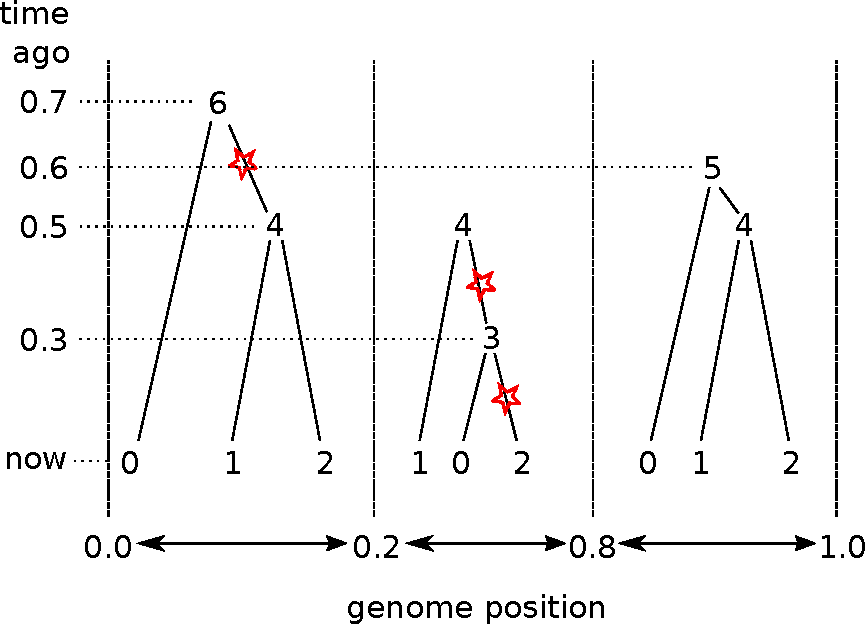
\includegraphics[width=0.6\textwidth]{example_tree_seq}
    \end{center}
    \caption{
        A pictorial representation of a tree sequence
        relating three samples to each other
        over a chromosome of length 1.0.
        Mutations shown in the example tables of the text
        are marked with red stars.
        \label{fig:ex_tree_seq}
    }
\end{figure}

To clarify terminology,
below a \emph{tree} refers to
a genealogical tree describing how a collection of individuals are related to each other.
A \emph{tree sequence} contains information sufficient to reconstruct the genealogical
tree relating all samples to each other at any point along the genome.
In the context of a tree sequence, \emph{nodes} refer to distinct ancestors,
and correspond to the vertices in the trees of a tree sequence.
Since each node represents a certain ancestor, it has a unique ``time'', thought of as her birth time,
which determines the height of any branching points she is associated with.  A given node will be
associated with branching points of all trees across a region if that node
is the most recent common ancestor to the subtending tips across that region.
This information is stored in the columns of a \textbf{Node Table}:
\begin{center}
\begin{tabular}{cccc}
    id   &  is\_sample &  population &  time \\
    0    &  1          & 0           & 0 \\
    1    &  1          & 0           & 0 \\
    2    &  1          & 0           & 0 \\
    3    &  0          & 0           & 0.3 \\
    4    &  0          & 0           & 0.5 \\
    5    &  0          & 0           & 0.6 \\
    6    &  0          & 0           & 0.7 \\
\end{tabular}
\end{center}
where ``flags'' records other information
(e.g., a binary mask of `1' indicates the node is a sample).
Importantly, the \textbf{node ID} of a node is given implicitly
by the (zero-based) index of its corresponding row in the Node Table.

Tree sequences are constructed by specifying over which segments of genome
which nodes inherit from which other nodes.  This information is stored by
recording the endpoints of each distinctly inherited ancestral segment,
the parental node, and a list of children nodes who have inherited that segment.
As each such record describes a collection of edges across a swatch of trees in the tree sequence,
we call these \emph{edgesets}
and store them in the columns of an \textbf{Edgeset Table:}
\begin{center}
\begin{tabular}{cccc}
    left & right & parent & children \\
    0.2  &  0.8  &  3     & 0,2 \\
    0.0  &  0.2  &  4     & 1,2 \\
    0.2  &  0.8  &  4     & 1,3 \\
    0.8  &  1.0  &  4     & 1,2 \\
    0.8  &  1.0  &  5     & 0,4 \\
    0.0  &  0.2  &  6     & 0,4  \\
\end{tabular}
\end{center}

To record information about genetic variants we need to also record each mutation
and which nodes have inherited that mutation.
The tree structure takes care of inheritance -- all we need to do
is to record the highest node in the tree at the mutated site
that inherited that mutation.
As more than one mtuation may occur at a given site,
we separate this information into two tables,
first, the \textbf{Site Table} records for each variant site
\begin{center}
\begin{tabular}{ccc}
    id  &   position  & ancestral\_state \\
    0   &  0.1        & 0 \\
    1   &  0.5        & 0 \\
\end{tabular}
\end{center}
Here ``position'' is a (floating point) position along the chromosome,
and ``ancestral state'' is the genotype of the root of the tree at that site.
As for nodes, \textbf{site IDs} are given implicitly
by the (zero-based) index of the rows.
Then, we record in a \textbf{Mutation Table}
\begin{center}
\begin{tabular}{ccc}
    site  & node  & derived\_state \\
    0	  & 4	  & 1 \\
    1	  & 3	  & 1 \\
    1	  & 2	  & 0 \\
\end{tabular}
\end{center}
in which ``site'' is the ID of the site at wihch this mutation occurred,
``node'' is the ID of the highest node that has inherited this mutation,
and ``derived state'' is the genotype at this site of any individuals inheriting this mutation,
unless another mutation occurs.
% \plr{Omit migrations?}

\paragraph{Definition of valid tables}
Here are the formal requirements for a set of nodes and edgesets to make sense,
and to allow ``msprime``'s algorithms to work properly.

To disallow time travel and multiple inheritance:
\begin{enumerate}
    \item Offspring must be born after their parents (and hence, no loops).
    \item The set of intervals on which each individual is a child must be disjoint.
\end{enumerate}
For algorithmic reasons, we also require:
\begin{enumerate} \setcounter{enumi}{2}
    \item The leftmost endpoint of each chromosome is 0.0.
    \item Node times must be strictly greater than zero.
    \item The list of offspring in an edgeset must be sorted.
    \item Edgesets must be sorted in nondecreasing time order.
    \item The set of intervals on which each individual is a parent must be disjoint.
    \item Each edgeset must contain at least two children.
\end{enumerate}
Note that since each node time is equal to the amount of time since the \emph{birth} of the
corresponding parent, time is measured in clock time, not in meioses.

A forwards-time simulation does \textbf{not} naturally emit genealogical information
satisfying requirements 5--8.
However, \msprime{} implements two algorithms that will take a set of tables
satisfying only 1--4 and produce tables satisfying all requirements.
Trivially, \texttt{sort\_tables} enforces requirements 5 and 6 and does not renumber nodes;
then, \texttt{simplify} enforces requirements 7 and 8 (and does much more; see below).


\section{More general method for recording the pedigree}

\plr{moved from above}

Concretely, this is done as follows.
Suppose that the forwards simulation algorithm labels (haploid) individuals by integers,
which we call ``input labels'',
to distinguish them from the ``node IDs'' given to these same individuals in the (output) tree sequence.
The algorithm maintains at all times a set of tables $(\nodes, \edgesets, \sites, \mutations)$
that record a relaxed tree sequence,
and an associative array $L$ that maps input labels to output node IDs, so that if $x$ is an input label,
then $L[x]$ is the corresponding output node ID.
We also always maintain $n$ to be the number of rows currently in the node table,
(so that with zero-indexed IDs, the next to be added will have node ID $n$),
$T_0$ to be the time of last simplification,
and $n_0$ the number of rows in the node table at that time.

Initially, we begin with $n$ and $n_0$ equal to the number of rows in the initial node table,
and $L[j] = i_j$ for each $0 \le j < N$ if the initial input generation is labeled
$i_0$, \ldots, $i_{N-1}$.

At a reproduction event where haploid parents $x$ and $y$ produce offspring $u$
at time $t$ in population $p$,
\begin{enumerate}
    \item add a
        $(
        \text{flags}=0,
        \text{population}=p,
        \text{time}=t)$ row to the node table,
    \item set $L[u] = n$,
    \item and increment $n\mathrel{+}=1$.
\end{enumerate}
Then, for each interval $[\ell,r)$ that $u$ inherits from parent $z$
(where $z$ is either $x$ or $y$),
\begin{enumerate}[resume]
    \item add a
        $( \text{left}=\ell,
        \text{right}=r,
        \text{parent}=z,
        \text{children}=(u,))$ row to the edgeset table.
\end{enumerate}
If furthermore there have been mutations at genomic locations $s_1$, \ldots, $s_k$
on this interval,
with derived states $q_1$, \ldots, $q_k$,
then for each $1 \le j \le k$,
\begin{enumerate}[resume]
    \item if $s_j$ is not in the site table, add a row
        $( \text{position}=s_j,
        \text{ancestral\_state}=0)$,
    \item find the site index $i$ whose position is $s_j$,
    \item and add a row
        $( \text{site}=i$,
           \text{node}=u$,
        \text{derived\_state}=q_j)$ to the mutation table.
\end{enumerate}

To \textbf{simplify} the tree sequence at time $T$,
\begin{enumerate}
    \item add $T-T_0$ to each time in the first $n_0$ rows of the node table,
        and replace each remaining time $t$ with $T-t$.
\end{enumerate}
Then, pass the set of currently alive input IDs,
$i_0, \ldots, i_{N-1}$ to the simplificaiton algorithm,
which produces a tree sequence that has node ID $j$ corresponding to input ID $i_j$
for $0 \le j < N$, and
\begin{enumerate}[resume]
    \item empty $L$,
    \item let $L[j] = i_j$ for $0 \le j < N$,
    \item set $n$ to be the number of nodes in the new tree sequence and set $n_0 = n$, and finally
    \item set $T_0 = T$.
\end{enumerate}

Simplification keeps the tables to a managable size.
Since the map $L$ is updated to maintain the association between individuals in the simulation
and nodes in the tree sequence, simplification can be run regularly,
as the simulation progresses.


\end{document}
